% !TeX program = xelatex
% ============================================================================
%  第 10 课　生成元、循环群与循环群的子群
% ----------------------------------------------------------------------------
%  编译        XeLaTeX，编译两遍
%  样式        ../../00-共享/preamble.tex
%  说明        本课不发单页（原 12+13 合并）
%  图片        圆盘类插图一律 \imgph 占位，不要在这里手画 tikz
% ============================================================================

\documentclass[10pt]{beamer}
% ============================================================================
%  讲义样式文件 —— 字体 / 配色 / 校徽栏 / 顶部导航栏 / 页脚 / 常用方框
%  所有个性化设置都集中在这里，改一次即可用于所有讲义
%
%  用法：主文件里写
%      \documentclass[10pt]{beamer}
%      \input{preamble.tex}
%  依赖：同目录下的 logo_white.png（顶部校徽）
%  编译：必须用 XeLaTeX，而且必须编译两遍
%        （顶部导航栏的节名与小圆点记录在 .nav 文件里，只编一遍不会更新）
% ============================================================================
\usepackage{ctex}  % 支持中文
\usepackage{amsmath, amssymb}  % 数学公式支持
\usepackage{fontspec}  % 字体设置
\usepackage{unicode-math}  % 支持Unicode数学字体
\usepackage{xcolor}  % 颜色
\usepackage{tikz}  % 用于绘制页脚色条
\usepackage{booktabs}  % 表格

% 图片搜索路径 ------------------------------------------------------------------
% 校本课的资料分目录存放，本文件可能被 02-课件/第XX课/ 、03-讲义/ 下的主文件调用，
% 这里把几种可能的相对位置都列上，logo_white.png 放在 00-共享/ 即可被找到。
% 最后一项 00-共享/图片/ 是给 \imgfig 用的插图目录（图与课件不在同一层，靠它找到）。
\graphicspath{{./}{./图片/}{../../00-共享/}{../00-共享/}{00-共享/}{../../00-共享/图片/}{../00-共享/图片/}{00-共享/图片/}}

% 设置字体
\setCJKmainfont{SimSun}  % 设置中文字体为宋体
\setmainfont{Palatino Linotype}  % 设置英文字体为Palatino Linotype
\setmathfont{Latin Modern Math}  % 设置数学字体为Latin Modern Math
% 注意：beamer 默认把正文字体族设成无衬线（sans），Windows 下对应的中文字体是
% 微软雅黑，所以上面这行 SimSun 目前对正文不起作用。想让正文变成宋体，取消
% 下面这行的注释即可（标题栏、页脚、方框标题不受影响）。
% \renewcommand{\familydefault}{\rmdefault}

% 定义颜色 - 均为绿色系
\definecolor{maingreen}{RGB}{34,139,34}  % 森林绿（导航栏底色）
\definecolor{lightgreen}{RGB}{240,255,240}  % 蜜瓜白（帧标题栏底色）
\definecolor{accentgreen}{RGB}{46,139,87}  % 海绿（强调色）
\definecolor{textgreen}{RGB}{0,128,0}  % 纯绿（标题文字）
\definecolor{darkgreen}{RGB}{20,90,20}  % 深绿（顶部校徽栏底色）

% 设置Beamer主题
\usetheme{default}
\usecolortheme{default}

% 自定义主题
\setbeamercolor{background canvas}{bg=white}
\setbeamercolor{frametitle}{fg=textgreen, bg=lightgreen}
\setbeamercolor{title}{fg=textgreen}
\setbeamercolor{subtitle}{fg=textgreen}
\setbeamercolor{section in toc}{fg=accentgreen}
\setbeamercolor{normal text}{fg=black}
\setbeamercolor{structure}{fg=accentgreen}
\setbeamercolor{itemize item}{fg=accentgreen}
\setbeamercolor{itemize subitem}{fg=accentgreen}
\setbeamercolor{itemize subsubitem}{fg=accentgreen}
\setbeamercolor{block title}{fg=white, bg=accentgreen}
\setbeamercolor{block body}{bg=lightgreen}
% example 环境（底层是 exampleblock）用的是独立的一组颜色名，default 配色主题下
% 它们的底色是空的，所以只设 block 的话“例”会变成一行没有框的标题，这里接过来
\setbeamercolor{block title example}{parent=block title}
\setbeamercolor{block body example}{parent=block body}

% ==================== 常用定理类方框（五类配色）====================
% 五类各自的标题条底色，正文底色由同色自动调浅（!8!white）
\definecolor{boxThm}{RGB}{20,90,20}    % 一、定理类：深绿
\definecolor{boxDef}{RGB}{46,139,87}   % 二、定义类：海绿
\definecolor{boxExm}{RGB}{34,139,34}   % 三、例题类：森林绿
\definecolor{boxPrf}{RGB}{85,107,47}   % 四、过程类：橄榄绿
\definecolor{boxNote}{RGB}{0,121,107}  % 五、注记类：青绿

% 方框本体：先套本类配色，再调用 beamer 的 block（改动只在环境内部生效）
\newcommand{\gbox}[2]{%
  \setbeamercolor{block title}{fg=white,bg=#1}%
  \setbeamercolor{block body}{bg=#1!8!white}%
  \begin{block}{#2}}
\newcommand{\gboxend}{\end{block}}
% 标题后的可选补充名：\begin{theorem}[勾股定理] → 定理（勾股定理）
\newcommand{\gsub}[1]{\ifx\relax#1\relax\else（#1）\fi}


% 一、定理类（定理/推论/性质/命题/引理）
\renewenvironment{theorem}[1][]{\gbox{boxThm}{定理\gsub{#1}}}{\gboxend}
\renewenvironment{corollary}[1][]{\gbox{boxThm}{推论\gsub{#1}}}{\gboxend}
\newenvironment{character}[1][]{\gbox{boxThm}{性质\gsub{#1}}}{\gboxend}
\newenvironment{proposition}[1][]{\gbox{boxThm}{命题\gsub{#1}}}{\gboxend}
\renewenvironment{lemma}[1][]{\gbox{boxThm}{引理\gsub{#1}}}{\gboxend}

% 二、定义类（定义/公理）
\renewenvironment{definition}[1][]{\gbox{boxDef}{定义\gsub{#1}}}{\gboxend}
\newenvironment{axiom}[1][]{\gbox{boxDef}{公理\gsub{#1}}}{\gboxend}

% 三、例题类（例/练习/习题）
\renewenvironment{example}[1][]{\gbox{boxExm}{例\gsub{#1}}}{\gboxend}
\newenvironment{exercise}[1][]{\gbox{boxExm}{练习\gsub{#1}}}{\gboxend}
\newenvironment{homework}[1][]{\gbox{boxExm}{习题\gsub{#1}}}{\gboxend}

% 四、过程类（证明/解/法1~法4）
\renewenvironment{proof}[1][]{\gbox{boxPrf}{证明\gsub{#1}}}{\qedsymbol\gboxend}
\newenvironment{jie}[1][]{\gbox{boxPrf}{解\gsub{#1}}}{\gboxend}
\newenvironment{way1}[1][]{\gbox{boxPrf}{法1\gsub{#1}}}{\gboxend}
\newenvironment{way2}[1][]{\gbox{boxPrf}{法2\gsub{#1}}}{\gboxend}
\newenvironment{way3}[1][]{\gbox{boxPrf}{法3\gsub{#1}}}{\gboxend}
\newenvironment{way4}[1][]{\gbox{boxPrf}{法4\gsub{#1}}}{\gboxend}

% 五、注记类（经验总结/注/值得注意的是/分析/提示）
\newenvironment{experience}[1][]{\gbox{boxNote}{经验总结\gsub{#1}}}{\gboxend}
\newenvironment{zhu}[1][]{\gbox{boxNote}{注\gsub{#1}}}{\gboxend}
\newenvironment{att}[1][]{\gbox{boxNote}{值得注意的是\gsub{#1}}}{\gboxend}
\newenvironment{analyse}[1][]{\gbox{boxNote}{分析\gsub{#1}}}{\gboxend}
\newenvironment{hint}[1][]{\gbox{boxNote}{提示\gsub{#1}}}{\gboxend}

% 顶部导航栏（miniframes 主题：显示各节名称 + 帧圆点）
% 节名与圆点记录在 .nav 文件中，改动章节后需要编译两遍才会同步
\useoutertheme[subsection=false]{miniframes}
\setbeamercolor{section in head/foot}{fg=yellow, bg=maingreen}
\setbeamercolor{mini frame}{fg=yellow, bg=maingreen}
\setbeamercolor{mini frame in current subsection}{fg=yellow, bg=accentgreen}

% 顶部校徽栏：位于导航栏上方，宽度与帧标题栏一致（整页宽）
% 校训用的楷体：ctex 的 \kaishu 在本机指向未安装的 Adobe 楷体，这里直接指定系统楷体
\setCJKfamilyfont{kaiti}{KaiTi}
\setbeamercolor{logo bar}{fg=white, bg=darkgreen}
\addtobeamertemplate{headline}{%
  \begin{beamercolorbox}[wd=\paperwidth,ht=0.84cm,dp=0.20cm,leftskip=0.25cm,rightskip=0.25cm]{logo bar}%
    % -0.035cm：色条内容默认坐在基线上，会比栏的中线略高，下移这一点使其上下居中
    \raisebox{-0.035cm}{
\includegraphics[height=0.72cm]{logo_white.png}}%
    % 右侧校训：字体为上面定义的楷体，也可改为 \insertsectionhead（当前节名）、\inserttitle（章节名）等
    % 0.375cm = 校徽中线（0.36cm）加汉字基线偏移，并同样下移 0.035cm 与校徽对齐
    \hfill\raisebox{\dimexpr 0.375cm - 0.5\height - 0.5\depth\relax}%
      {\CJKfamily{kaiti}\fontsize{12pt}{24pt}\selectfont 自强不息，止于至善}%
  \end{beamercolorbox}%
}{}

% % 设置边框 - 使用TikZ绘制圆角
% \setbeamertemplate{frametitle}{
%   \vspace*{0.2cm}
%   \begin{tikzpicture}
%     % 背景矩形宽度限制为标题内容宽度
%     \fill[lightgreen, rounded corners=5pt] (0,0) rectangle (\textwidth+0.6cm, 0.8cm);
%     \node[anchor=west, text width=\textwidth, xshift=0.3cm, yshift=0.4cm] {\usebeamerfont{frametitle}\insertframetitle};
%   \end{tikzpicture}
% }

% 设置项目符号
\setbeamertemplate{itemize item}{\small\raise0.5pt\hbox{\textcolor{accentgreen}{$\bullet$}}}
\setbeamertemplate{itemize subitem}{\small\raise0.3pt\hbox{\textcolor{accentgreen}{$\circ$}}}

% 设置页脚 - 使用TikZ绘制一条整页宽的色条，左侧页码、右侧姓名
\setbeamertemplate{footline}{
  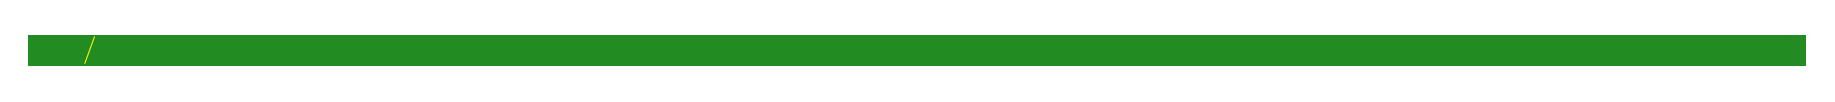
\begin{tikzpicture}
    \fill[maingreen] (-1,0) rectangle (\paperwidth, 0.4cm);
    \node[yellow,anchor=east, xshift=0cm, yshift=0.2cm] {\insertframenumber/\inserttotalframenumber};
    % 原点在纸张左边缘右侧 1cm 处（色条从 x=-1cm 画起），故 \paperwidth-2cm
    % 对应纸张右边缘内缩 1cm 的位置，与左侧页码左右对称
    \node[yellow,anchor=east, xshift=\paperwidth-2cm, yshift=0.2cm] {\insertauthor};
  \end{tikzpicture}
}

% 关闭 beamer 默认的导航符号（页码与姓名已在页脚中自行绘制）
\setbeamertemplate{navigation symbols}{}

% 设置标题页面
\setbeamertemplate{title page}{
  \vspace{0.5cm}
  \begin{center}
    \begin{minipage}[c][0.68\paperheight][c]{\textwidth}
      {\usebeamerfont{title}\usebeamercolor[fg]{title}\large\inserttitle\par}
      \vspace{1.5cm}
      {\usebeamerfont{subtitle}\usebeamercolor[fg]{subtitle}\Large\insertsubtitle\par}
      \vspace{1.5cm}
      {\usebeamerfont{author}\usebeamercolor[fg]{author}\insertauthor\par}
      \vspace{0.5cm}
      {\usebeamerfont{institute}\usebeamercolor[fg]{institute}\insertinstitute\par}
      \vspace{0.5cm}
      {\usebeamerfont{date}\usebeamercolor[fg]{date}\insertdate\par}
    \end{minipage}
  \end{center}
}

% 设置块环境
\setbeamertemplate{blocks}[rounded][shadow=false]

% 设置目录
\setbeamertemplate{section in toc}{\inserttocsectionnumber.~\inserttocsection}


% ----------------------------------------------------------------------------
%  图片占位符（临时用；有图以后把那行换成 \includegraphics 即可）
%      \imgph{说明文字}          默认高 3.6cm
%      \imgph[6cm]{说明文字}     指定高度
%  会画一个绿色虚线框，框里写说明，方便对着 PDF 找位置。
\newcommand{\imgph}[2][3.6cm]{%
  \begin{center}%
  \begin{tikzpicture}%
    \node[draw=accentgreen, densely dashed, line width=1pt, rounded corners=4pt,
          fill=lightgreen, inner sep=8pt, align=center, text width=0.72\textwidth,
          minimum height=#1, font=\small]
      {\textcolor{accentgreen}{\bfseries 【图片占位】}\\[4pt] #2};%
  \end{tikzpicture}%
  \end{center}%
}

% ----------------------------------------------------------------------------
%  插图（图已就位后用这个；图放在 00-共享\图片\ 下，由 \graphicspath 找到）
%      \imgfig{文件名}                 默认宽 0.72\textwidth
%      \imgfig[0.55\textwidth]{文件名}  指定宽度
%      \imgfig[8cm]{文件名}            也可以直接给尺寸
%  图源与编译方法见 00-共享\图片\README.md。每张图是一页 PDF，只含图、无页边。
\newcommand{\imgfig}[2][0.72\textwidth]{%
  \begin{center}%
    \includegraphics[width=#1]{#2}%
  \end{center}%
}

% ----------------------------------------------------------------------------
%  可用方框环境速查（五类配色，均不编号，均支持 \begin{xxx}[补充名]）
%    定理类（深绿）  theorem 定理 / corollary 推论 / character 性质 /
%                    proposition 命题 / lemma 引理
%    定义类（海绿）  definition 定义 / axiom 公理
%    例题类（森林绿）example 例 / exercise 练习 / homework 习题
%    过程类（橄榄绿）proof 证明 / jie 解 / way1 法1 / way2 法2 /
%                    way3 法3 / way4 法4
%    注记类（青绿）  experience 经验总结 / zhu 注 / att 值得注意的是 /
%                    analyse 分析 / hint 提示
%  另有 beamer 自带的普通方框：\begin{block}{标题} ... \end{block}
% ----------------------------------------------------------------------------


% ==================== 每份课件只改这一段 ====================
\title{从数数开始的抽象代数生活}
\subtitle{第 10 课　生成元、循环群与循环群的子群}
\author{姜博瀚}
\institute{厦门大学附属实验中学}
\date{\today}
% ============================================================

\begin{document}

\begin{frame}
  \titlepage
\end{frame}

% ============================================================================
\section{什么是生成}

\begin{frame}{回顾：八个动作，两个就够}
  上节课的最后一句：\(D_4\) 的 \(8\) 个动作，只要 \(r\)（转 \(90^\circ\)）和 \(f\)（翻一次）就够。
  \pause
  \begin{center}
    其余六个怎么来？\pause 用 \(r\) 和 \(f\) 反复复合出来：
    \[
      r^2=rr,\qquad r^3=rrr,\qquad rf,\qquad r^2f,\qquad r^3f .
    \]
  \end{center}
  \pause
  \begin{center}
    {\large 今天把这个「够用」，说成一个定义。}
  \end{center}
\end{frame}

\begin{frame}{由 a 生成的子群}
  \begin{definition}[由 \(a\) 生成的子群]
    在群 \(G\) 里，把元素 \(a\) 和它反复做出来的所有结果放在一起，
    得到的那个小群，叫做\textbf{由 \(a\) 生成的子群}，记作 \(\langle a\rangle\)。
  \end{definition}
  \pause
  \begin{definition}[生成元、循环群]
    如果整个群 \(G\) 能由一个元素 \(a\) 生成，也就是 \(G=\langle a\rangle\)，
    就说 \(a\) 是 \(G\) 的一个\textbf{生成元}，而 \(G\) 是一个\textbf{循环群}。
  \end{definition}
\end{frame}

% ============================================================================
\section{模 12 加法里的生成元}

\begin{frame}{从 0 开始，一直加 3}
  \[
    0 \to 3 \to 6 \to 9 \to 12 \to \cdots
  \]
  \pause
  走到 \(12\) 就等于回到 \(0\)。所以一直加 \(3\) 只能圈住这几个：
  \[
    \langle 3\rangle=\{0,\ 3,\ 6,\ 9\} .
  \]
  \pause
  \begin{center}
    一共 \(4\) 个。\quad 它跑不出这 \(4\) 个。
  \end{center}
\end{frame}

\begin{frame}{换 5 试试}
  \[
    0 \to 5 \to 10 \to 3 \to 8 \to 1 \to 6 \to 11 \to 4 \to 9 \to 2 \to 7 \to 0
  \]
  \pause
  \begin{center}
    {\large 一直加 \(5\)，把 \(12\) 个数一个不落地全走了一遍。}
  \end{center}
  \pause
  \begin{center}
    {\large 所以 \(5\) 是模 \(12\) 加法的一个生成元，\\
    这个群 \(\langle 5\rangle=\{0,1,2,\dots,11\}\) 是循环群。}
  \end{center}
\end{frame}

\begin{frame}{为什么 3 只圈住 4 个，5 却圈住 12 个？}
  \begin{center}
  \begin{tabular}{@{}lcc@{}}
    \toprule
     & \(3\) 和 \(12\) 的公因数 & 圈住几个 \\
    \midrule
    \(3\) & \(1,3\)（最大的是 \(3\)） & \(12\div3=4\) \\
    \(5\) & 只有 \(1\) & \(12\div1=12\) \\
    \bottomrule
  \end{tabular}
  \end{center}
  \pause
  \begin{center}
    {\large 公因数越大，圈住的越少。\quad 只有公因数 \(1\) 时，整整一圈都被圈住。}
  \end{center}
  \pause
  \begin{att}
    这和第 3 课是同一件事。第 3 课讲的是模 \(7\) 的乘法（人人有逆元）和模 \(6\) 的乘法（\(2\) 没有）；
    换成模 \(12\) 也一样：和 \(12\) 只有公因数 \(1\) 的数，才有逆元。
  \end{att}
\end{frame}

\begin{frame}{用手指回答}
  \begin{itemize}
    \item \(\langle 2\rangle\) 里有几个数？是哪几个？
    \item \(\langle 6\rangle\) 里有几个数？是哪几个？
    \item \(7\) 是模 \(12\) 加法的生成元吗？
  \end{itemize}
  \pause
  \begin{block}{答案}
    \(6\) 个：\(\{0,2,4,6,8,10\}\)；\quad \(2\) 个：\(\{0,6\}\)；\quad 是（\(7\) 和 \(12\) 只有公因数 \(1\)）。
  \end{block}
\end{frame}

% ============================================================================
\section{元素的阶，就是生成子群的大小}

\begin{frame}{数的阶：反复加自己，几次回到 0}
  \begin{center}
  \begin{tabular}{@{}l*{12}{c}@{}}
    \toprule
    \(a\) & 1 & 2 & 3 & 4 & 5 & 6 & 7 & 8 & 9 & 10 & 11 & 0 \\
    \midrule
    阶 & 12 & 6 & 4 & 3 & 12 & 2 & 12 & 3 & 4 & 6 & 12 & 1 \\
    \bottomrule
  \end{tabular}
  \end{center}
  \pause
  \begin{center}
    {\large 全班一起报，老师填表。}
  \end{center}
  \pause
  \begin{center}
    {\large 这和三角形里「做几次回到不动」是同一件事，只是把动作换成了数。}
  \end{center}
  \pause
  \begin{theorem}[阶与生成子群]
    元素 \(a\) 的阶，正好等于由它生成的子群 \(\langle a\rangle\) 的大小。
  \end{theorem}
\end{frame}

\begin{frame}{用手指回答}
  \begin{itemize}
    \item \(4\) 的阶是多少？\(\langle 4\rangle\) 里有几个数？
    \item \(8\) 的阶是多少？\(\langle 8\rangle\) 和 \(\langle 4\rangle\) 是同一个子群吗？
  \end{itemize}
  \pause
  \begin{block}{答案}
    \(3\) 个：\(\{0,4,8\}\)；\quad 也是 \(3\)，\(\langle 8\rangle=\{0,8,4\}\)，和 \(\langle 4\rangle\) 一模一样。
  \end{block}
\end{frame}

% ============================================================================
\section{循环群里的所有小圈}

\begin{frame}{把能自成一体的小圈都圈出来}
  \begin{center}
  \begin{tabular}{@{}clc@{}}
    \toprule
    子群 & 是谁 & 大小 \\
    \midrule
    \(\{0\}\) & 只有 \(0\) & \(1\) \\
    \(\{0,6\}\) & 加 \(6\) 来回走 & \(2\) \\
    \(\{0,4,8\}\) & 由 \(4\) 生成 & \(3\) \\
    \(\{0,3,6,9\}\) & 由 \(3\) 生成 & \(4\) \\
    \(\{0,2,4,6,8,10\}\) & 由 \(2\) 生成 & \(6\) \\
    \(\{0,1,2,\dots,11\}\) & 全部十二个 & \(12\) \\
    \bottomrule
  \end{tabular}
  \end{center}
  \pause
  \begin{center}
    {\large 没有别的小圈了——一共就这 \(6\) 个。}
  \end{center}
\end{frame}

\begin{frame}{大小都是 12 的因数}
  \begin{center}
    {\Large \(1,\ 2,\ 3,\ 4,\ 6,\ 12\)}
  \end{center}
  \pause
  \begin{center}
    {\large 每一个都能整除 \(12\)——一个例外都没有。}
  \end{center}
  \pause
  \begin{att}
    \(S_3\) 里是 \(1,2,3,6\) 整除 \(6\)；\(D_4\) 里是 \(1,2,4,8\) 整除 \(8\)；
    这里是 \(1,2,3,4,6,12\) 整除 \(12\)。三张纸上，同一句话。
  \end{att}
\end{frame}

\begin{frame}{这节课要带走的三句话}
  \begin{itemize}
    \item \textbf{生成元}：一个元素反复做，能造出整个群，就叫生成元；这样的群叫\textbf{循环群}。
    \item 元素的\textbf{阶} \(=\) 由它生成的子群的大小。
    \item 循环群的子群大小，一定能整除整个群的大小。
  \end{itemize}
  \pause
  \begin{center}
    {\large\textcolor{textgreen}{\bfseries 下节课：回头去看幂的尾巴——它会转圈。}}
  \end{center}
\end{frame}

% ---------------- 结尾页 ----------------
\begin{frame}
  \begin{center}
    \vspace{1.6cm}
    {\Large\textcolor{textgreen}{\bfseries 下课}}

    \vspace{1.0cm}
    {\large\textcolor{accentgreen}{下节课：幂的尾巴转圈了——从现象到猜想}}
  \end{center}
\end{frame}

\end{document}